\documentclass[12pt,a4paper]{article}
\usepackage[utf8]{inputenc}
\usepackage[spanish]{babel}
\usepackage{amsmath}
\usepackage{amsfonts}
\usepackage{amssymb}
\usepackage{makeidx}
\usepackage{graphicx}
\usepackage{lmodern}
\usepackage{kpfonts}
\usepackage{fourier}
\usepackage[left=2cm,right=2cm,top=2cm,bottom=2cm]{geometry}
\author{Rodriguez Lopez Francisco Javier}
\begin{document}

\begin{center}
\LARGE \textbf{Universidad Politecnica de la Zona Metropoilitana de Guadalajara\\}



\includegraphics[scale=1]{Upzmg5.png} 

\large \textbf{Giro de un motor de corriente directa}\\
\vspace{2cm}
\large \textbf{Nombre: Rodriguez Lopez Francisco Javier.\\
\vspace{0.5cm} Matricula: 18311804.\\
\vspace{0.5cm} Carrera: Ingenieria en Mecatronica.\\
\vspace{0.5cm} Materia: Sistemas Electronicos de Interfaz.\\
\vspace{0.5cm} Curso: septiembre-diciembre del 2019.\\
\vspace{0.5cm} Docente: Moran Garabito Carlos Enrique.}


\vspace{6cm}
\small \textbf{15 de Octubre del 2019}
\end{center}

\section{Motor de Corriente Directa:}

Se sabe que la especialidad del motor electrico, es convertir ese tipo de energia a energia mecanica, esto debido a las bobinas que trae consigo en su interior, para despues crear un campo magnetico, que excite dichas bobinas, para despues de eso, empezar con la rotacion que es nuestro punto a ver en este tema.\\
En todo caso, al pasar al momento en el que este emerge a la excitacion de las bobinas, este es reflejado en unos imanes que trae consigo en su interior, para posterior de ello trabajar, como estos lo hacen, atrayendose algunos polos con otros, y viceversa, es decir polo positivo con polo positivo, se juntan, creando un rechazamiento, que esto genera mas fuerza y dezplazamiento en el motor, lo que lo hace de alguna forma hacer la rotacion necesaria para que el motor funcione.\\
Este tipo de motores, son los mas concurrentes y por ende mas usados, puesto que son los que generan menos energia y su uso es bastante amplio, en cuestion estos son muy utilizados, en muchos de los electrodomesticos que se pueden observar en un hogar. El funcionamiento se basa en la interacción entre el campo magnético del imán permanente y el generado por las bobinas, ya sea una atracción o una repulsión.\\

\begin{figure}[hbtp]
\centering
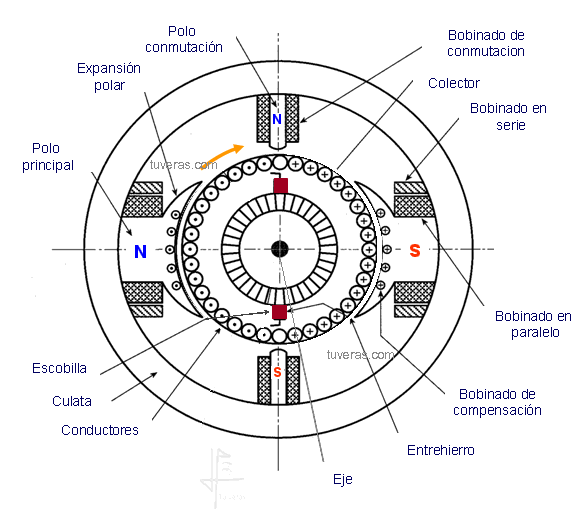
\includegraphics[width=8cm]{Motor2.png}
\caption{Vista de las partes del motor}
\end{figure}


Entrando a temas mas especificos, como lo es el de la bobina, este tiene en si en su interior un nucleo, este nucleo es el que genera el movimiento del motor, conocido como torque, en este punto se reconoce que hay polos del mismo signo trabajando a lapar,para que estos hagan una repulsion de fuerzas electromagneticas, y de ese modo ese rechazo, genere elgiro, y en un modo la fuerza de este, siendo estos entre mas excitado, mas fuerte su campo magnetico y en constancia la fuerza con la que se genera el torque de este motor.\\
En esta instancia es factible ver el modo en que el torque puede ser calculado, esto para ver su velocidad entre otras caracteristicas, que nos dejan ver la potencia de nuestro motor.\\

$$ t=Fl=rF sen°=F_{tan}*r $$

En todo caso, el momento del torque es el que nos deja definir de mejor estancia, el trabajo de nuestro giro.\\
Existen otras formulas, para el ver el trabajo del motor.\\
Potencia:
$$ P=t*w $$
Momento angular y Momento de inercia
$$ L=I*w $$ $$ I=m*r^{2} $$
Velocidad Angular:
$$ w=\frac{0}{t} $$
Velocidad tangencial:
$$ v_{tan}=\frac{2\pi r}{T} $$
Trabajo:
$$ W=\dfrac{1}{2}Iw^{2} $$

Cada una de las formulas son fundamentales, para ver el progreso que tendra nuestro motor, en este calculo se ve solo lo dinamico, mas que nada para hacer correr el motor, de buena forma y que este no pueda inferir en cuestiones como desgaste, u otros factores que hacen de estos motores, eficientes.\\

\textbf{Funcionamiento:}\\
En general, los motores de corriente continua son similares en su construcción a los generadores. De hecho podrían describirse como generadores que funcionan al revés. Cuando la corriente pasa a través del rotor de un motor de corriente continua, se genera un par de fuerzas por la reacción magnética, y el rotor gira. La acción del conmutador y de las conexiones de las bobinas del campo de los motores son exactamente las mismas que usan los generadores. La revolución del rotor induce un voltaje en las bobinas de ésta. Este voltaje es opuesto en la dirección al voltaje exterior que se aplica a el rotor, y de ahí que se conozca como voltaje inducido o fuerza contraelectromotriz.\\

Cuando el motor gira más rápido, el voltaje inducido aumenta hasta que es casi igual al aplicado. La corriente entonces es pequeña, y la velocidad del motor permanecerá constante siempre que el motor no esté bajo carga y tenga que realizar otro trabajo mecánico que no sea el requerido para mover el rotor. Bajo carga, el rotor gira más lentamente, reduciendo el voltaje inducido y permitiendo que fluya una corriente mayor en el rotor. El motor puede
así recibir más potencia eléctrica de la fuente, suministrándola y haciendo más trabajo mecánico. Debido a que la velocidad de rotación controla el flujo de la corriente en el rotor, deben usarse aparatos especiales para arrancar los motores de corriente continua. Cuando el rotor está parada, ésta no tiene realmente resistencia, y si se aplica el voltaje de funcionamiento normal, se producirá una gran corriente, que podría dañar el conmutador y las bobinas del rotor. El medio normal de prevenir estos daños es el uso de una resistencia de encendido conectada en serie a el rotor, para disminuir la corriente antes de que el motor consiga desarrollar el voltaje inducido adecuado. Cuando el motor acelera, la resistencia se reduce gradualmente, tanto
de forma manual como automática \cite{pernia2011conceptos} .\\

\begin{center}
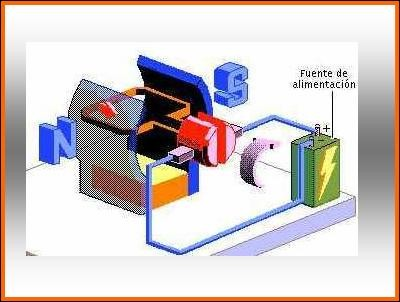
\includegraphics[width=10cm]{Motor.png}
\end{center}


La velocidad a la que funciona un motor depende de la intensidad del campo magnético que actúa sobre el rotor, así como de la corriente de ésta.
Cuanto más fuerte es el campo, más bajo es el grado de rotación necesario para generar un voltaje inducido lo bastante grande como para contrarrestar el voltaje aplicado. Por esta razón, la velocidad de los motores de corriente continua puede controlarse mediante la variación de la corriente del campo.\\
Los carbones cierran el circuito de la fuente con las dos delgas y la espira conectada a ellas, de esta forma circula corriente por las espiras, como esto ocurre dentro de un campo magnético, aparecen fuerzas sobre las espiras y el rotor comienza a girar.

En cuestiones de desarrollo, para el buen giro del motor se debe de ver la velocidad proporcionada por la tension aplicada:\\
$$ U= (R*I)+E $$
Siendo estos:
\begin{itemize}
\item U:Tension media aplicada.
\item R*I:Caida de tension, debido al factor corriente.
\item E:Fuerza electromotriz inducida.
\end{itemize}

Para tener mas en cuenta el giro del rotor, daddo el campo magnetico, tenemos que tener en cuenta, el tipo de excitacion que se esta teniendo de por medio para la corriente llegada a la bobina, y que este genere el necesario, para las funciones que nosotros necesitemos y con cuanta fuerza.\\

\textbf{Excitacion de Iman permanente:} Este tipo de excitacion, es de las mas eficientes, ya que su entrada no esta predestinada por la corriente que vaya a llegar a su nucleo, sino que su nucleo no necesita de energia electrica en su devanado, ya que este ya trae en si el tipo de excitacion que lo reserva, esto para no dejar a la deriva solo la excitacion propia del nucleo, sino que esto lo beneficia en potencia, y en durabilidad.\\

\textbf{Excitacion Independiente:} Este tipo de excitaciones, dan gran prestigio ya que en su nucleo se puede tener control sobre la parte de inductor, como por el inducido, siendo este a la regulacion mas exacta y de mayor rendimiento, para que al momento de llegar al campo magnetico, se pueda tener un buen torque, y un buen giro del motor, para que todo este en dependencia del control y de la corriente dada en tiempos.
Conformados por:\\
\begin{itemize}
\item Electromagnetico.
\item Iman permanente.
\end{itemize}

\textbf{Autoexcitacion:} Este tipo de excitacion, es de las mas conflicitvas, de manejar gracias a su necesidad de tener una fuente de eenrgia externa al circuito del motor, conllevado a ser de los mas lentos, este tipo de excitaciones es tambien de las mas utilizadas, en algunos casos, pero se debe de tener en cuenta el grosor del cobre y la durabilidad que tendra este al paso de la corriente, entre otros factores, que en si son muy utilizados.
Conformados por:\\
\begin{itemize}
\item Motor en serie.
\item Motor en parelo.
\item Motor Compound.
\end{itemize}

\bibliographystyle{apalike}
\bibliography{ref}

\end{document}